\section{Arhitectura DVM versiunea 2}

Cea de-a doua versiune a \gls{dvm} a fost implementată pentru a treia demonstraţie de concept a rețelelor de transport de date fără fir desfăşurată în cadrul \gls{onf} \cite{onf2016_poc3}. A fost dezvoltată pe scheletul primei versiuni, păstrând aceeaşi abordare: un server \gls{netconf} care se bazează pe soluţia software \textit{OpenYuma} și un fişier de configurare din care serverul poate citi valori pentru atributele \gls{yang} pe care le expune. Din acest punct de vedere, \gls{dvm} versiunea 2 folosește întregul model informațional pentru microunde TR-532 și o parte semnificativă din modelul informațional de bază, TR-512.1, cumulând aproximativ 300 de astfel de parametri.

Arhitectura celei de-a doua versiuni a \gls{dvm} este influenţată de natura atributelor \gls{yang} ce alcătuiesc modelul informațional pentru microunde \cite{stancu2017enabling}: parametri de configurare, de stare sau care prezintă capabilitățile dispozitivului. Atributele de configurare pot fi citite sau scrise și prin intermediul acestora un utilizator poate influenţa comportamentul dispozitivului. Parametrii de stare pot fi doar citiţi și reprezintă situația curentă a echipamentului, în timp ce capabilitățile sunt atribute care pot fi doar citite și descriu abilităţile dispozitivului.

Mediatorul cu valori implicite a fost gândit astfel încât să fie flexibil și să ofere posibilitatea înlocuirii citirii valorilor din fişierul de configurare cu o citire dintr-un echipament real, cu ajutorul unui protocol la alegere. Deoarece mediatorul este o aplicație software externă, care nu face parte din echipamentele de transport de date fără fir, în momentul inițializării ar trebui să reflecte configurația echipamentului la care se conectează. Din cauza faptului că dispozitivul nu are o configuraţie statică și aceasta poate fi modificată înaintea inițializării mediatorului, nu poate fi utilizată baza de stocare de date de iniţializare oferită de serverul \gls{netconf}. Asta înseamnă ca în momentul inițializării mediatorul trebuie să își construiască baza de stocare de date de operare într-un mod arborescent, interogând dispozitivul de rețea asupra valorilor atributelor. Acest lucru se aplică doar în cazul parametrilor configurabili sau în cazul celor care au un caracter static, precum capabilitățile echipamentului. Deoarece aceste valori se salvează în baza de stocare de date de operare, înseamnă că acestea nu sunt persistente și vor fi citite la fiecare iniţializare din dispozitiv. Fiindcă simulatorul \gls{dvm} a fost proiectat ca un mediator real, toate aceste aspecte se reflectă și în arhitectura acestuia, diferenţa fiind că valorile atributelor nu se citesc dintr-un dispozitiv, ci dintr-un fişier de configurare descris în limbajul \gls{xml}.

Natura atributelor \gls{yang}, descrisă anterior, a dus la arhitectura celei de-a doua versiuni a \gls{dvm}, care se poate vedea în Figura \ref{fig:dvm_v02_architecture}. Atributele \gls{yang} au fost împărţite în trei categorii: de iniţializare, de execuţie și de configurare.

\begin{figure}[h]
	\centering
	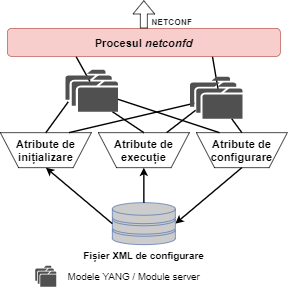
\includegraphics{dvm_v02_architecture}
	\caption{Arhitectura simulatorului DVM versiunea 2.}
	\label{fig:dvm_v02_architecture}
\end{figure}

Parametrii de iniţializare reprezintă acele atribute statice, care sunt citite din dispozitiv o singură dată, în momentul inițializării simulatorului. În cadrul serverului \gls{netconf} pot fi doar citite, în cazul parametrilor care reprezintă capabilitățile echipamentului (adică informaţie statică, prezentată de către dispozitiv, care nu se poate schimba) sau pot fi și scrise și citite, ca în cazul parametrilor de configurare. În momentul inițializării \gls{dvm} aceștia sunt consideraţi parametri de pornire, ca apoi să devină de configurare, având câte o funcție cu apel invers asociată, care permite modificarea acestei valori în fişierul \gls{xml} de configurare prin intermediul serverului \gls{netconf}. Nu este nevoie ca aceste atribute de configurare să fie citite din dispozitiv decât în momentul inițializării, deoarece apoi se presupune că orice configurare a dispozitivului se va face prin echipamentul de control \gls{sdn}, deci prin intermediul serverului \gls{netconf} care va fi astfel informat asupra noii valori a parametrilor respectivi.

Atributele de execuţie reprezintă parametrii dinamici ai dispozitivului, care pot fi doar citiţi, precum alarme, informații de stare sau de monitorizare a performanţelor. Acestea trebuie citite din echipament de fiecare dată când controlerul \gls{sdn} le cere, din cauza naturii lor dinamice. Soluția acestei abordări constă în nodurile virtuale oferite de soluția \textit{OpenYuma}. În loc de a avea o valoare stocată pentru un atribut \gls{yang}, sau valori pentru grupuri de atribute, \textit{OpenYuma} oferă posibilitatea de a asocia o funcție cu apel invers pentru astfel de parametri. Aceasta va fi apelată de fiecare dată când valoarea atributului asociat este cerută serverului \gls{netconf}, iar implementarea acesteia va prelua valoarea din fişierul \gls{xml} de configurare, sau va construi arborele asociat răspunsului, în cazul unui grup de atribute.

Cea de-a doua versiune a simulatorului \gls{dvm} se bazează pe abordarea \textit{OpenYuma} de a folosi funcții cu apel invers pentru implementarea funcţionalităţii de citire sau scriere asociată atributelor modelelor \gls{yang} \cite{openyuma2012qsg}. Proiectarea \gls{dvm} urmăreşte separarea descrisă anterior a parametrilor, oferind diferite funcții cu apel invers pentru diferitele categorii. Fiecare atribut din modelele \gls{yang} va fi reprezentat ca un nod \textit{OpenYuma}, care reprezintă un tip de date pus la dispoziţie de această soluție software, conţinând diverse informații rezultate din analizarea modelului \gls{yang}, precum numele, constrângeri asupra valorilor pe care atributul le poate lua și funcţia cu apel invers asociată, de citire sau de scriere. Astfel, au fost considerate trei funcții cu apel invers generice, care să fie folosite în cele trei cazuri date de împărțirea atributelor \gls{yang}: pentru parametrii de iniţializare, de execuţie și de configurare. Acestea sunt considerate generice, deoarece o singură astfel de funcție cu apel invers este utilizată pentru fiecare tip de atribut, diferenţierea pentru fiecare atribut în parte făcându-se în implementarea acesteia, în funcție de numele atributului. Această abordare oferă flexibilitate și uşurinţă în implementarea simulatorului \gls{dvm}.

